
Tabular data, including product descriptions and features, is a major component of e-commerce, although natural language is used for most user interactions, such as Q\&A and helper agents. The need for models that can efficiently interpret tabular data and engage consumers through logical, context-aware communication is thus urgent.
\\

In order to meet this need, table-to-text creation is essential, particularly in e-commerce, where it makes it possible to provide user-specific summaries, customized descriptions, and product reviews. The ability to convert structured patient records into succinct summaries for physicians \citep{he2023survey} and turn tabular financial data into analytical reports \citep{Varshney_2024} are two examples of industries that possess this capability in addition to e-commerce. Despite its benefits, creating text that is both comprehensible and appropriate for the context from structured data is still quite difficult, especially when coordinating input data and goal outputs with user-specific needs.
\\

User or query-centric scenarios, which require high-quality datasets that capture domain-specific perspectives, exacerbate these difficulties. The depth needed for specialized applications such as product reviews is typically absent in existing table-to-text datasets, which tend to concentrate on general-purpose summaries \citep{macková2023promapdatasetsproductmapping}. The utility of datasets such as QTSUMM \citep{zhao2023qtsummqueryfocusedsummarizationtabular} for attribute-specific product reviews is limited because they provide tabular summaries that are unrelated to the product domain. Product-specific text production, on the other hand, needs to take into account a variety of characteristics (such as battery life and display quality) and adjust to different user intents, including offering technical details or condensed pros and drawbacks.
\begin{figure}[H]
    \centering
    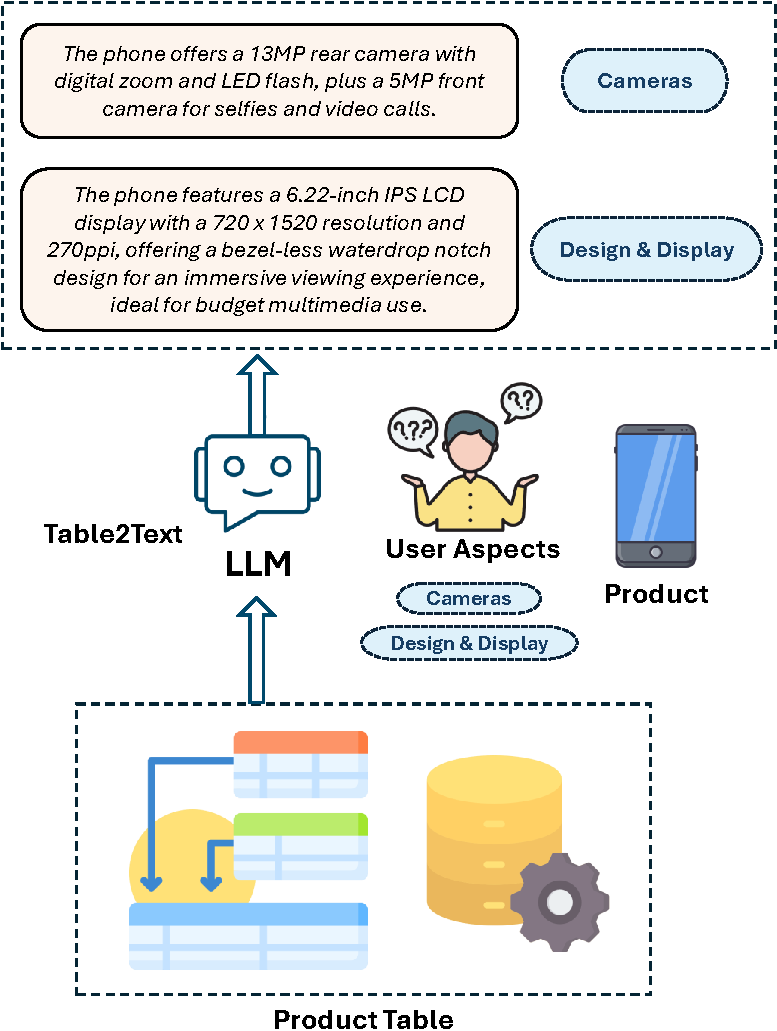
\includegraphics[scale = 0.60]{images/task-def.pdf}
    \caption{Product Table2Text}
    \label{fig:task-def}
\end{figure}
The challenges of generating text from tables have been present in several studies. Fine-tuned models like LLama2-chat \citep{jiang2023mistral} and StructLM \citep{gao2024jsontuning} have improved performance on table-based datasets by using training data tailored to specific domains. Meanwhile, general-purpose LLMs like GPT-4 and BERT have shown impressive capabilities in generating text \citep{openai2024gpt4technicalreport, devlin2019bertpretrainingdeepbidirectional}. However, creating attribute-specific text for complex e-commerce tasks requires customized datasets, as current methods struggle with the unique demands of product-related domains.
\\

Some progress has been made with datasets designed for table-to-text tasks, like ROTOWIRE \citep{wiseman2017challengesdatatodocumentgeneration}, TabFact \citep{2019TabFactA}, and WikiTableT \citep{chen2021wikitabletlargescaledatatotextdataset}. For example, ROTOWIRE generates sports summaries, TabFact supports fact-checking, and WikiTableT focuses on creating descriptions from Wikipedia tables. But these datasets don't provide the depth needed for generating product-specific text. Other datasets, such as ToTTo \citep{parikh2020tottocontrolledtabletotextgeneration} and LogicNLG \citep{chen2020logicalnaturallanguagegeneration}, focus on logical deductions and advanced sentence generation but they still not significant for product-related tasks. The growing need for domain-specific datasets tailored to product reviews and attribute-based summaries has been underscored by recent research \citep{He2023ReviewOS}.
\\

This paper introduces a table-to-text dataset for the products domain and explores whether fine-tuned LLMs can bridge the gap between general-purpose capabilities and domain-specific needs in e-commerce. By leveraging tailored datasets and fine-tuning techniques, this work seeks to empower e-commerce platforms to generate more precise and engaging product reviews, enhancing customer satisfaction and business outcomes.
